\section{Dominoes}

(Partial) lock rule? Constructible configurations.

\subsection{Tetris with vertical dominoes}

Using the introduced notation, the problem is $\textsc{Tetris-NoRotation}\lbrack \VD \rbrack $ both \clearing and \survival. The input consist of sequence of vertical dominoes and an arbitrary sized $n \times m$ board in a contractible configuration.

\subsubsection{Constructible board configurations}

First we will to characterize the contractible boards with $\VD$ pieces without rotation by exploring the configuration starting from an empty board. Vertical dominoes consist of two vertical adjacent cells. 

For an empty board, any trajectory fixes the piece in the bottom row, filling $\cell[1][i]$ and $\cell[2][i]$ cells for any $1 \leq i \leq m$. The next domino can either go to an empty column or to the one before. Placing the first $m$ dominoes in unfilled columns clears the two lowest rows, and consequently the board. When a domino is placed in a non-empty column $i$, the $\cell[3][i]$ and $\cell[3][i]$ are filled, and so on util a $\VD$ is placed in the last unfilled column. When this happens the two lowest rows are cleared and the process continues. 

So we can represent a reachable configuration of a given $n \times m$ board $B$ with a sequence of $m$ integers $(a_1, \dots, a_m)$, where

$$0 \leq a_i \leq \lceil \frac{n}{2} \rceil, \;\;\;   \forall i = 1,\dots, m$$

and $\exists i$ such that $a_i = 0$, with the following mapping: 

$$
\cell = \begin{cases}
   \text{filled}  & \text{if } i \leq  2a_j  \\
   \text{empty}   & \text{if } i >  2a_j
\end{cases}
$$

Each $a_i$ counts the number of vertical pieces placed in the column $i$. For example, in a $10 \times 6 $  board, the sequence $(1,2,0,4,2,3)$ defines the configuration in 
\ref{dom:vconf}.

\begin{figure}[h]\label{dom:vconf} 
    \centering
    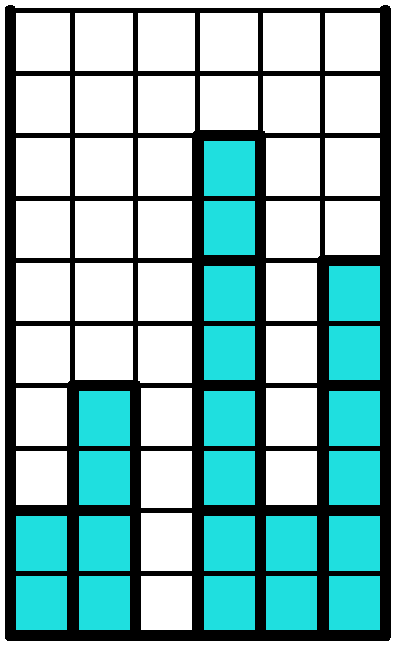
\includegraphics[width=0.2\textwidth]{./pictures/dominoes/vertical_configuration.pdf}
    \caption{The $10 \times 6 $ board configuration represented by the sequence $(1,2,0,4,2,3)$.}
\end{figure}

\subsubsection{Cleaing}

The input is a 
